\section{Ejecta Dynamicss}

% =========================================================
\begin{frame}{Dynamics}

\begin{columns}[t]

% ----- Left column -----
\column{0.5\textwidth}
\centering

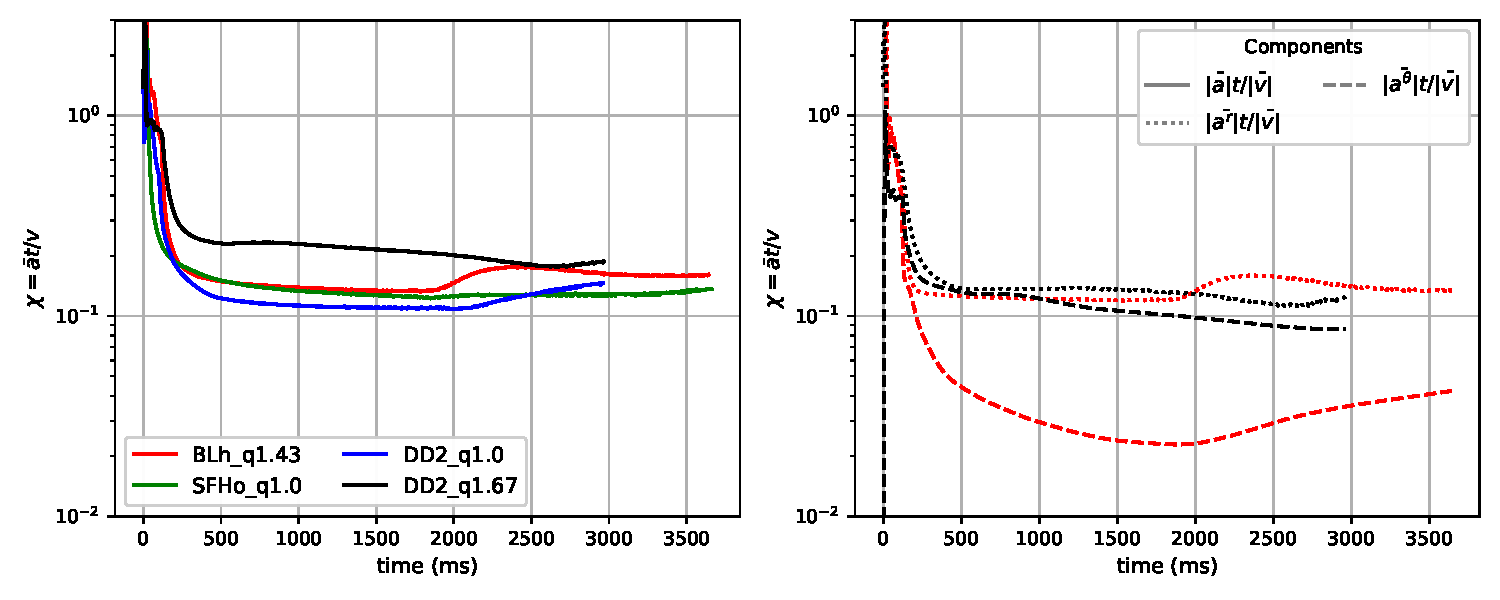
\includegraphics[width=\linewidth]{../fig/model_comparison/Chi_joined.pdf}

\vspace{-0.3em}

\hspace{0.15\linewidth}%

\includegraphics[width=0.7\linewidth]{../fig/model_comparison/Expansion_and_heating_energies_v3.pdf}

% ----- Right column -----
\column{0.5\textwidth}

\begin{itemize}\scriptsize
    \item $\chi \equiv \bar{a} t / v$
    \item All models show decaying $\chi$ after the end of injection
    \item Models show increasing $\chi$ at $t \sim 2\,\mathrm{s}$
    \begin{itemize}\scriptsize
        \item Due to mass exiting the grid
    \end{itemize}
    \item DD2\_q1.67 has significant non-radial motion
    \begin{itemize}\scriptsize
        \item Due to elevated nuclear heating
    \end{itemize}
\end{itemize}

\vspace{0.5em}

\centering
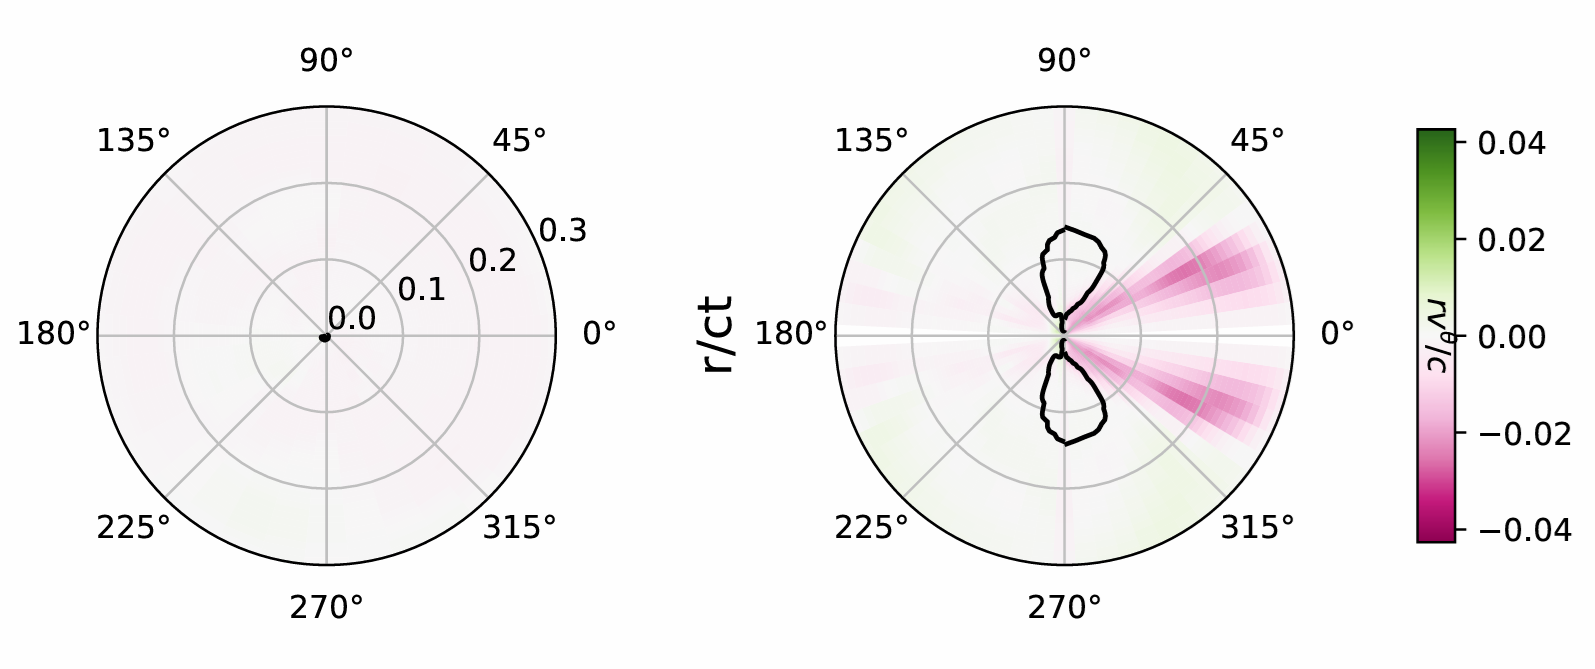
\includegraphics[width=\linewidth]{../fig/dd2_180_vlr_hr_constatm/velocities_final_cropped.png}

\end{columns}
\end{frame}

% =========================================================
\begin{frame}{Dynamics}

\begin{columns}[t]

% ----- Left column -----
\column{0.5\textwidth}
\centering


\includegraphics[width=\linewidth]{../fig/dd2_180_vlr_hr_constatm/HRdens_final.pdf}

% ----- Right column -----
\column{0.5\textwidth}

\begin{itemize}\scriptsize
    \item $\chi \equiv \bar{a} t / v$
    \item All models show decaying $\chi$ after the end of injection
    \item Models show increasing $\chi$ at $t \sim 2\,\mathrm{s}$
    \begin{itemize}\scriptsize
        \item Due to mass exiting the grid
    \end{itemize}
    \item DD2\_q1.67 has significant non-radial motion
    \begin{itemize}\scriptsize
        \item Due to elevated nuclear heating
    \end{itemize}
\end{itemize}

%\vspace{0.5em}

%\centering
%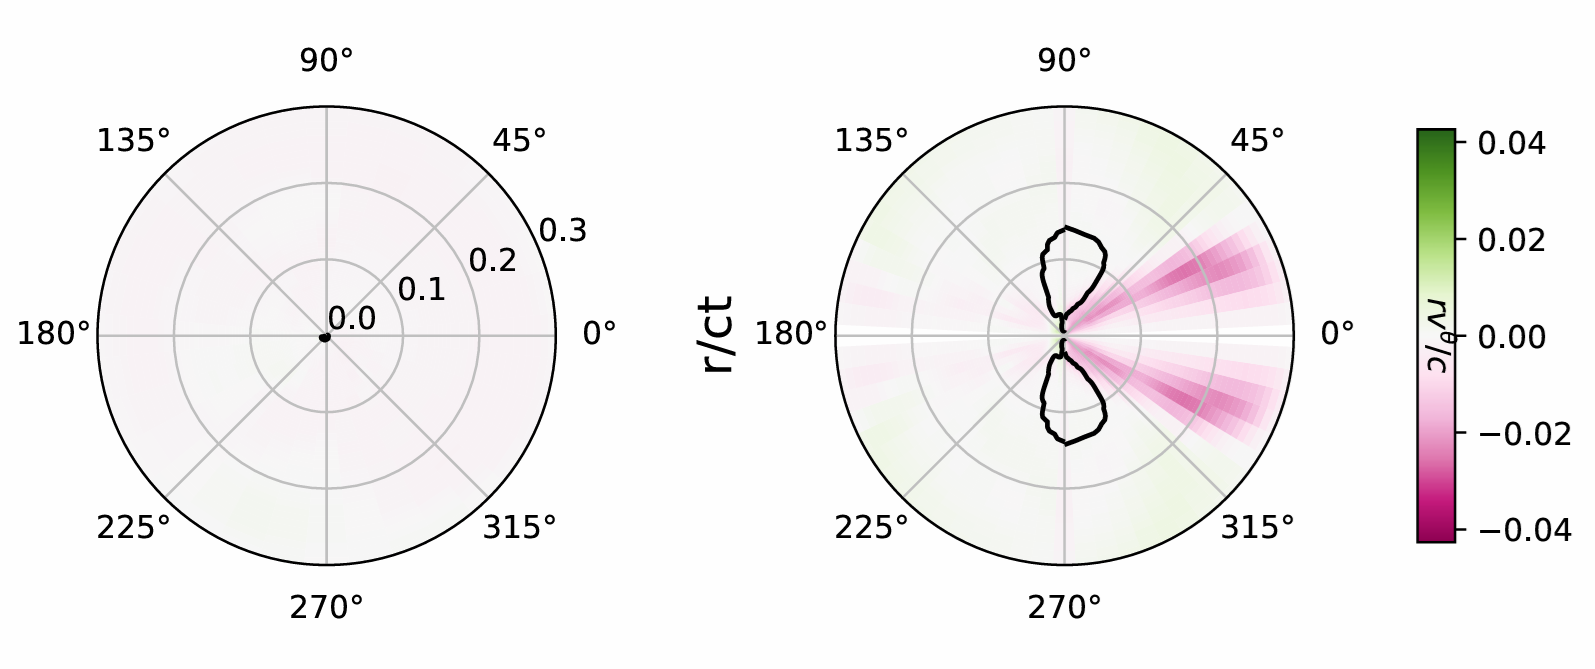
\includegraphics[width=\linewidth]{../fig/dd2_180_vlr_hr_constatm/velocities_final_cropped.png}

\end{columns}
\end{frame}

% =========================================================
\begin{frame}{Fallback material}

\begin{columns}[t]

% ----- Left column -----
\column{0.5\textwidth}

\begin{itemize}\scriptsize
    \item Estimated fallback mass
    \item Only SFHo\_q1.0 includes ejection in NR
    \item SFHo\_q1.0 has a disk mass $M \sim 0.011\,M_{\odot}$ (Gutiérrez et al.\ 2025)
    \item Viscous disk ejecta $\sim 30\%$ of disk mass (Fujibayashi et al.\ 2020)
    \item Possible interaction between these components
\end{itemize}

\vspace{0.5em}

\scriptsize
\begin{tabular}{c|c|c}
\hline\hline
Model & $M_{\mathrm{fall}}\,[M_{\odot}]$ & $M_{\mathrm{ej}}\,[M_{\odot}]$ \\
\hline\hline
BLh\_q1.43 & $1.24\times10^{-3}$ & $7.33\times10^{-3}$ \\
SFHo\_q1.0 & $1.17\times10^{-3}$ & $4.12\times10^{-3}$ \\
DD2\_q1.0  & $7.79\times10^{-4}$ & $4.14\times10^{-3}$ \\
DD2\_q1.67 & $3.99\times10^{-3}$ & $1.27\times10^{-2}$ \\
\hline\hline
\end{tabular}



% ----- Right column -----
\column{0.5\textwidth}


\centering
\begin{tikzpicture}
    % Main (centered) figure
    \node (main) {
        
\includegraphics[width=1.0\linewidth]{../fig/model_comparison/Mejecta_time_evolution_joined.pdf}
    };

    % Inset figure (top-right corner)
    \node[
        anchor=north east,
        xshift=0.6em,
        yshift=2.0em
    ] at (main.north east) {
        
\includegraphics[width=0.5\linewidth]{../fig/sfho_vlr_hr_constatm/Mass_injection.pdf}
    };
\end{tikzpicture}



\end{columns}
\end{frame}
